\chapter{Yara}
\label{sec:yara}

\emph{Yara} (\emph{Y}et \emph{a}nother \emph{r}ead \emph{a}ligner) is an exhaustive, non-heuristic read mapper, capable of quickly reporting all stratified mapping locations within a given error rate.
Yara works with Illumina or Ion Torrent reads, supports paired-end and mate-pair protocols, computes accurate mapping qualities, offers parallelization via multi-threading, has a low memory footprint thanks to the FM-index, and does not require ad-hoc parameterization.

% -----------------------------------------------------------------------------

\section{Engineering}
\label{sec:yara:eng}

\subsection{Adaptive filtration}
\label{sec:yara:eng:adaptive}

Specific yet rapid filtration is fundamental in the design of an efficient read mapping tool.
Read mappers like RazerS\,3 \citep{Weese2012} and mrFast \citep{Ahmadi2012} are designed around na\"ive filtration with exact seeds.
This filtration method is always very quick, however it is not specific enough on long, repetitive reference genomes like the human genome.
Masai \citep{Siragusa2013} circumvents this problem by enforcing a minimum seed length,
whose optimal value must be tuned for a specific reference genome, and eventually resorting to approximate seeds in order to guarantee full-sensitivity.
This filtration method speeds up Masai by an order of magnitude but has some drawbacks:
it needs external parametrization, lacks flexibility and is suboptimal in practice.

Yara applies an adaptive filtration scheme \emph{per read} because, under any fixed filtration scheme, the number of verifications per read is not uniform: within a typical human genome resequencing, most reads produce very few verifications and are easily mappable, while few other reads are problematic and often not even confidently mappable to one single location.
Consequently, any fixed filtration scheme turns out to be too weak for some reads yet too strong for others, thus suboptimal in practice.
An adaptive filtration scheme per read improves filtration efficiency by optimizing the ratio between filtration speed and specificity.
Yara thus automatically chooses an adaptive filtration scheme per read, without requiring manual parameterization by the user.

Adaptive filtration works as follows.
Yara initially applies filtration with exact seeds to all reads.
The tool counts the number of verifications to be performed for each read, thus decides if it is worth proceeding with the verification phase or alternatively applying a stronger filtration scheme.
This decision depends on fine-tuned internal verification thresholds.
Under standard Illumina setups, exact seeds provide efficient filtration for up to 70--80\,\% of the reads; on the remaining reads, a filtration scheme using $1$-- or $2$--approximate seeds works better.
Thus, Yara starts with the quickest filtration scheme and becomes more specific whenever it pays off to do so.

%For instance, when mapping 100\,bp Illumina reads on the human genome within 5\,\% error rate, filtration with exact seeds produces 6 exact seeds of length 16\,bp;
%under these terms, a single read produces an average of 15000 verifications, and the verification phase takes 99\,\% of the runtime.
%On the same mapping setup, this method produces 3 $1$--approximate seeds of length 33\,bp; thus a single read produces 1400 verifications on average.
%Under this setup, Masai in all-mapping still spends about 20\,\% of its runtime in filtration and the remaining 80\,\% in verification.
%The next stronger filter produces 2 $2$--approximate seeds of length 50\,bp.

\subsection{Stratified mapping}
\label{sec:yara:eng:strata}

All-mapping methods consider a set of relevant mapping locations per read.
Yet, this definition leaves open what relevant means.
In all-mapping under the edit distance, the user defines relevant mapping locations by imposing a distance threshold.
Despite being sound, this definition does not work well in practice.
On the one hand a very low threshold leaves a consistent fraction of the reads unmapped, on the other hand a moderate threshold produces a deluge of mapping locations for some reads.
In practice, at 5\,\%, error rate, Illumina reads map on average to hundreds of mapping locations on the human genome.
It is questionable whether all these locations are relevant for the downstream analysis.
Thus, a finer definition of all-mapping relevance is necessary in practice.

%\subsubsection{Stratified mapping}

Stratification of mapping locations yields an equally sound yet practical definition of all-mapping under the edit distance.
The $e$-stratum
\begin{eqnarray}
S(r,e) = \{ (i,j,e) : d_E(g_{i \dots j},r) = e\}
\end{eqnarray}
denotes the set of all mapping locations of a read $r$ at edit distance $e$ from the reference genome $g$.
According to the above definition, conventional all-mapping under the edit distance defines the set
\begin{eqnarray}
S(r,0) \cup S(r,1) \cup \dots \cup S(r,k)
\end{eqnarray}
as relevant mapping locations within an \emph{absolute} error threshold $k$.
Stratified all-mapping refines this definition by considering only mapping locations being co-optimal, or sub-optimal up to a certain degree.
Formally, if the distance of any optimal mapping location for read $r$ is
\begin{eqnarray}
e^* = \min \,\{ e \in [0,k] : S(r,e) \neq \emptyset \}
\end{eqnarray}
stratified all-mapping considers mapping locations
\begin{eqnarray}
S(r,e^*) \cup \dots \cup S(r,\min \,\{ e^*+l, k\})
\end{eqnarray}
within a \emph{relative} error threshold $l$ to be relevant.
%Note that $l \ll k$.

\subsubsection{Efficient filtration by strata}

Yara significantly improves the runtime of stratified all-mapping over conventional all-mapping.
Obviously, the most straightforward way to achieve stratified all-mapping consists into performing conventional all-mapping and subsequently filtering out any irrelevant mapping location.
For instance, RazerS\,3 implements this method and gets no speedup.
Another na\"ive method consists into applying up to $k$ rounds of conventional all-mapping, using filtration schemes for thresholds going from $0$ to $\min \,\{ e^*+l, k\}$.
It is easy to see that also this method performs redundant computation: the total work for any read that maps at distance greater or equal to $k$ corresponds to the sum of all $k$ filtration schemes.

The following stratified all-mapping method, implemented in Yara, guarantees not to perform more work than conventional all-mapping.
Indeed, the key idea is to simply reduce any filtration scheme full-sensitive within distance $k$ to be full-sensitive within distance $\min \,\{ e^*+l, k\}$.
Given a filtration scheme $\mathbf{t}=(t_1,\dots,t_s)$ full-sensitive within distance $k$, any subset consisting of $s^* \leq s$ seeds with thresholds $\mathbf{t^*}=(t^{*}_{1},\dots,t^{*}_{s^*})$ is full-sensitive within distance $\min \,\{ e^*+l, k\}$ if it satisfies
\begin{eqnarray}
s^* + \sum_{i=1}^{s^*} t_i^* > \min \,\{ e^*+l, k\}.
\end{eqnarray}
%The proof is analogous to that one given in section~\ref{sec:seeds-apx}.
%Verification of all candidate locations produced by one seed or by one threshold accounts for one stratum $S(r,i)$.

\begin{example}
Let $k=5$ be the absolute threshold, and $l=0$ be the relative threshold, restricting relevant locations to co-optimal ones.
A read $r$ maps at distance 1, \ie $|S(r,0)| = 0$ and $|S(r,1)| > 0$, thus $e^* = 1$.
Given the filtration scheme $\mathbf{t}=(1,1,1)$, any subset full-sensitive up to distance $\min \,\{ e^*+l, k\} = 1$ finds all relevant mapping locations.
All full-sensitive subsets of $\mathbf{t}$ are $(0,0,-)$, $(0,-,0)$, $(-,0,0)$, $(1,-,-)$, $(-,1,-)$, $(-,-,1)$, where a $-$ at position $i$ indicates that the $i$-th seed is unnecessary.
Thus, the verification of all candidates, either produced by \emph{any} two exact seeds or by one 1-approximate seed, yields all mapping locations in the $1$-stratum of $r$.
\end{example}

\subsubsection{Greedy verification strategy}

In addition, Yara implements a simple greedy strategy to minimize the number of verifications necessary to find all relevant stratified mapping locations.
As candidate locations can be verified in any order, Yara chooses an ordering of seeds producing the minimum number of verifications.
The tool first finds all seeds and ranks them by number of candidate locations produced.
Then it processes all candidate locations, from the least to the most frequent seed, until it explores $l$ strata from the first non-empty one, or until it attains the absolute distance threshold $k$.

Yara performs best-mapping by means of stratified filtration.
Best-mapping requires one primary mapping location along with its confidence.
Under the edit distance, without any further assumptions, any co-optimal location is equally likely to be correct.
Thus, Yara performs stratified all-mapping with a relative threshold $l=0$, picks one random co-optimal location, and subsequently estimates its mapping quality using all found mapping locations (see section~\ref{sec:yara:eng:qualities}).
Thanks to this method, Yara in best-mapping is an order of magnitude faster than in all-mapping.

% Yara uses the best strata
%(i) to compute precise mapping qualities
%(ii) to perform paired-end mapping.


\subsection{Paired-end and mate-pair protocols}
\label{sec:yara:eng:pairs}
Paired-end and mate-pair protocols are the sequencing protocols of choice of Illumina instruments.
Reads are sequenced in pairs from both ends of the same insert.
Properly paired reads are expected to map within the insert size adopted in the sequencing protocol.
Thus, the added information of an expected insert size allows a read mapper to map read pairs to their original locations more confidently than in the single-end protocol.
Nonetheless, a read mapper should report equally important unpaired mapping locations, as the lack of any proper pair of mapping locations signals a potential structural variation, \eg a long indel or an inversion.

In the paired-end or mate-pair workflows, Yara maps paired reads independently, exactly as in the single-end workflow, and reports all relevant mapping locations per read.
However, in addition to the single-end workflow, Yara implements a finer strategy to choose primary mapping locations.
For any reads pair, among all pairs of co-optimal mapping locations, the tool selects the one with minimal deviation from the expected insert size.
Since Yara outputs all relevant mapping locations, the choice of primary locations can be always corrected a posteriori.

\subsection{Mapping qualities}
\label{sec:yara:eng:qualities}
Yara computes mapping qualities using the number of mapping locations stratified by error rate.
%Mapping quality for the paired-end and mate-pair protocols.

\subsection{Indexing}
\label{sec:yara:eng:indexing}

Yara uses an efficient FM-index specialization for the DNA alphabet, based on interleaved rank dictionaries (see section~\ref{sec:index:succinct:rd}).
This interleaved FM-index exhibits a fourfold speedup over the first FM-index implementation bundled with Masai.
Surprisingly, the interleaved FM-index is also faster than any other index, both in exact and approximate search (see section~\ref{sec:index:algo}).
Moreover, this index consumes only 1.23 bytes per base pair with a SA sampled at 10\,\%, thus its memory footprint for the human genome is 3.7~GB.
Under these terms, there is no space-time indexing trade-off: the FM-index always provides the most convenient suffix trie implementation.

Yara does not use the multiple search algorithms of section~\ref{sec:index:algo:multimismatch} to search seeds on the FM-index.
As shown in section~\ref{sec:index:algo}, on the FM-index it is always faster to search exact queries in a na\"ive way and approximate queries after sorting them in lexicographical order.
This fact considerably simplifies a fine-grained parallelization of the tool.

%Yara implements fine-grained parallelism.
%It would be possible to stream over reads to parallelize computation per read.
%However, the tool processes batches of reads.

% -----------------------------------------------------------------------------

\section{Evaluation}
\label{sec:yara:eval}

The evaluation consists of three experiments, all using the human reference genome (GRCh37).
The first experiment assesses all-mapping sensitivity by applying the Rabema benchmark on real data.
The second experiment evaluates best-mapping accuracy on simulated data.
The last experiment assesses the performance of best-mappers within a variant calling pipeline applied to real data.
In addition, all above experiments track runtimes and memory consumptions.

%Experiment measure read mapping throughput in \emph{giga base pairs per hour} (Gbp/h).
%The Illumina HiSeq\,2500 in a six days run produces\footnote{According to the specifications at \url{http://res.illumina.com/documents/products/datasheets/datasheet_hiseq2500.pdf} for high output run mode with dual flow cell.} up to 800~Gbp as $2 \times 100\,\text{bp}$ paired-end reads.
%Under this measure the maximum throughput of the Illumina HiSeq\,2500 is $5.56$ Gbp/h.
%Runtimes for each tool are measured on de-facto standard input and output formats, \ie they consider the time to produce a compressed BAM file from a gzipped FastQ file.

I compared Yara to the following state-of-the-art tools: Bowtie\,2, BWA, GEM, RazerS\,3, and Hobbes\,2.

\subsection{Experimental setup}

\subsubsection{Read mappers parametrization}

In appendix \ref{sup:yara:param}, I give the exact parametrization of each read mapper considered in the evaluation.
Whenever possible, I configured the tools with the appropriate error rate (Yara, GEM, RazerS\,3) or absolute number of errors (Hobbes\,2).
When processing paired-end reads, I provided the tools with appropriate insert size information.

\subsubsection{Infrastructure}

All tools run on a desktop computer running Linux~3.10.11, equipped with one Intel\textsuperscript{\textregistered} Core i7-4770K CPU @ 3.50\,GHz, 32\,GB RAM and a 2\,TB HDD @ 7200\,RPM.
For maximum throughput, all tools run using eight threads.
For accurate running time comparisons, I disabled Intel Turbo Boost; therefore, all measured running times might be slightly higher than the actual ones.

\subsection{Rabema benchmark on real data}

The first experiment evaluates the sensitivity of all-mapping on real data through the Rabema benchmark.
The \emph{Rabema benchmark} \citep{Holtgrewe2011} (v1.1) measures the sensitivity of read mappers in finding \emph{relevant} mapping locations of genomic reads.
This experiment considers the Rabema benchmark categories \emph{all} and \emph{all-best}.
In the category all, Rabema counts as relevant, for each read, all mapping locations within a maximal edit distance error rate; in the category all-best it considers just co-optimal mapping locations.
Rabema computes the \emph{sensitivity} of each tool as the fraction of relevant mapping locations found per read.
For a thorough evaluation, Rabema classes mapping locations by their \emph{error rate}, then computes sensitivity within each error rate class.
The benchmark reports percentual scores normalized by the number of reads.

The data used in this experiment is a publicly released sequencing run (SRA/ENA id: ERR161544) by the Beijing Genome Institute;
the genomic DNA used in this study came from an anonymous male Han Chinese individual who has no known genetic diseases.
This dataset consists of $2 \times 100\,\text{bp}$ whole genome sequencing reads produced by an Illumina HiSeq 2000 instrument.
For practical reasons, in the category \emph{all-best} I consider the first $10\,\text{M}$ reads, while in the category \emph{all} the first $1\,\text{M}$ reads.

I run the Rabema benchmark within an error rate of 5\,\%, as it is sufficient to map almost all reads in the dataset.
Therefore, I built a Rabema gold standard by running RazerS\,3 in full-sensitive mode up to 5\,\% error rate.
Subsequently, I provided unpaired reads to each tool as the Rabema benchmark, by definition, does not consider paired-end reads.
Results are shown in table~\ref{tab:yara:rabema}.

\begin{table*}[t]
  \caption[Yara results in the Rabema benchmark]
  {
  \label{tab:yara:rabema}
    Rabema benchmark results on the human reference genome.
    The left panel shows the results of mapping $1\,\text{M}$ Illumina-like $2 \times 100\,\text{bp}$ simulated reads; the right panel shows the results of mapping $1\,\text{M}$ Illumina $2 \times 100\,\text{bp}$ real reads.
    Big numbers show total Rabema scores, while small numbers show marginal scores for the mapping locations at
    $\bigl(\begin{smallmatrix}\mbox{\tiny 0}&\mbox{\tiny 1}&\mbox{\tiny 2}\\\mbox{\tiny 3}&\mbox{\tiny 4}&\mbox{\tiny 5}\end{smallmatrix}\bigr)$ \% error rate.
    }
  \vspace{-3mm}
  \center
  \sffamily
  \resizebox{0.95\textwidth}{!}
  {
	\renewcommand{\tabcolsep}{0.8ex}
	% latex table generated in R 3.0.3 by xtable 1.7-1 package
% Thu Jun 12 14:19:45 2014
\begin{tabular}{llcccccc}
  \toprule
  & \multirow{2}{*}{}  &\multicolumn{ 3 }{c}{  hiseq\_hg19\_like } &\multicolumn{ 3 }{c}{  ERR161544 } \\
  &&\multicolumn{3}{c}{H.\,sapiens}&\multicolumn{3}{c}{H.\,sapiens} \\
  \cmidrule(lr){3-5}\cmidrule(lr){6-8} 
  & tool  &\multicolumn{1}{c}{  all } &\multicolumn{1}{c}{  all-best } &\multicolumn{1}{c}{  any-best } &\multicolumn{1}{c}{  all } &\multicolumn{1}{c}{  all-best } &\multicolumn{1}{c}{  any-best } \\
    \midrule
\multirow{4}{*}{\begin{sideways}best\quad\ \end{sideways}} &  Yara  & \cellcolor[rgb]{0.720936613806026,0.693912049872418,0.500586753718633}\phantom{0}92.09 {\subcolbeg\begin{tabular}{rrr} \cellcolor[rgb]{0.403921568627451,0.713725490196078,0.549019607843137}\phantom{}100.00 & \cellcolor[rgb]{0.491934846520128,0.708224660327786,0.535573134831756}\phantom{0}97.99 & \cellcolor[rgb]{0.917167406257914,0.681647625344175,0.470607049316261}\phantom{0}85.94\\ \cellcolor[rgb]{0.953766814861723,0.492673421065653,0.48503605221722}\phantom{0}40.28 & \cellcolor[rgb]{0.952944439300722,0.482393726553148,0.48626961555872}\phantom{0}10.10 & \cellcolor[rgb]{0.952941189897827,0.482353109016955,0.486274489663063}\phantom{00}2.56\subcolvspace\\\end{tabular}\subcolend} & \cellcolor[rgb]{0.403941544585273,0.713724241698715,0.549016555960692}\phantom{}100.00 {\subcolbeg\begin{tabular}{rrr} \cellcolor[rgb]{0.403921568627451,0.713725490196078,0.549019607843137}\phantom{}100.00 & \cellcolor[rgb]{0.403921568627451,0.713725490196078,0.549019607843137}\phantom{}100.00 & \cellcolor[rgb]{0.403921568627451,0.713725490196078,0.549019607843137}\phantom{}100.00\\ \cellcolor[rgb]{0.403921568627451,0.713725490196078,0.549019607843137}\phantom{}100.00 & \cellcolor[rgb]{0.406558070018315,0.713560708859149,0.548616809019533}\phantom{0}99.94 & \cellcolor[rgb]{0.416936311515842,0.712912068765554,0.5470312443463}\phantom{0}99.71\subcolvspace\\\end{tabular}\subcolend} & \cellcolor[rgb]{0.403935126998755,0.713724642797872,0.549017536425299}\phantom{}100.00 {\subcolbeg\begin{tabular}{rrr} \cellcolor[rgb]{0.403921568627451,0.713725490196078,0.549019607843137}\phantom{}100.00 & \cellcolor[rgb]{0.403921568627451,0.713725490196078,0.549019607843137}\phantom{}100.00 & \cellcolor[rgb]{0.403921568627451,0.713725490196078,0.549019607843137}\phantom{}100.00\\ \cellcolor[rgb]{0.403921568627451,0.713725490196078,0.549019607843137}\phantom{}100.00 & \cellcolor[rgb]{0.406558070018315,0.713560708859149,0.548616809019533}\phantom{0}99.94 & \cellcolor[rgb]{0.411546262160783,0.713248946850245,0.547854724108878}\phantom{0}99.83\subcolvspace\\\end{tabular}\subcolend} & \cellcolor[rgb]{0.77612231864183,0.69046294332018,0.492155604368718}\phantom{0}90.49 {\subcolbeg\begin{tabular}{rrr} \cellcolor[rgb]{0.403921568627451,0.713725490196078,0.549019607843137}\phantom{}100.00 & \cellcolor[rgb]{0.627201181679237,0.699770514380342,0.514907444738003}\phantom{0}94.64 & \cellcolor[rgb]{0.963223148104967,0.61087758660621,0.470851552352353}\phantom{0}75.66\\ \cellcolor[rgb]{0.954931478025793,0.507231710616531,0.483289057471114}\phantom{0}50.19 & \cellcolor[rgb]{0.953225730320086,0.485909864295192,0.485847679029675}\phantom{0}30.86 & \cellcolor[rgb]{0.952954192257764,0.48251563851617,0.486254986123158}\phantom{0}14.27\subcolvspace\\\end{tabular}\subcolend} & \cellcolor[rgb]{0.404232490103558,0.713706057603822,0.548972105950954}\phantom{0}99.99 {\subcolbeg\begin{tabular}{rrr} \cellcolor[rgb]{0.403921568627451,0.713725490196078,0.549019607843137}\phantom{}100.00 & \cellcolor[rgb]{0.403921568627451,0.713725490196078,0.549019607843137}\phantom{}100.00 & \cellcolor[rgb]{0.403995038035294,0.713720898358088,0.549008383350272}\phantom{}100.00\\ \cellcolor[rgb]{0.405930939290696,0.713599904529626,0.548712620658475}\phantom{0}99.96 & \cellcolor[rgb]{0.409374614123684,0.713384674852564,0.548186503670102}\phantom{0}99.88 & \cellcolor[rgb]{0.430690965543723,0.712052402888811,0.544929838869818}\phantom{0}99.40\subcolvspace\\\end{tabular}\subcolend} & \cellcolor[rgb]{0.40417027268568,0.713709946192439,0.548981611389797}\phantom{0}99.99 {\subcolbeg\begin{tabular}{rrr} \cellcolor[rgb]{0.403921568627451,0.713725490196078,0.549019607843137}\phantom{}100.00 & \cellcolor[rgb]{0.403921568627451,0.713725490196078,0.549019607843137}\phantom{}100.00 & \cellcolor[rgb]{0.403921568627451,0.713725490196078,0.549019607843137}\phantom{}100.00\\ \cellcolor[rgb]{0.405765129581401,0.713610267636457,0.548737952697395}\phantom{0}99.96 & \cellcolor[rgb]{0.408474724554735,0.713440917950623,0.548323986798691}\phantom{0}99.90 & \cellcolor[rgb]{0.424930592809047,0.712412426184729,0.545809895815394}\phantom{0}99.53\subcolvspace\\\end{tabular}\subcolend} \\ 
    &  Gem  & \cellcolor[rgb]{0.662487413804443,0.697565124872516,0.509516492607764}\phantom{0}93.71 {\subcolbeg\begin{tabular}{rrr} \cellcolor[rgb]{0.403921568627451,0.713725490196078,0.549019607843137}\phantom{}100.00 & \cellcolor[rgb]{0.460059300512323,0.710216881953274,0.540443009916282}\phantom{0}98.73 & \cellcolor[rgb]{0.762955649856365,0.691285860119271,0.494167178766498}\phantom{0}90.88\\ \cellcolor[rgb]{0.957368599070872,0.537695723680024,0.479633375903495}\phantom{0}61.29 & \cellcolor[rgb]{0.953249434251992,0.486206163444023,0.485812123131815}\phantom{0}31.48 & \cellcolor[rgb]{0.952957090382862,0.482551865079895,0.486250638935511}\phantom{0}15.01\subcolvspace\\\end{tabular}\subcolend} & \cellcolor[rgb]{0.404281727902643,0.713702980241379,0.548964583509427}\phantom{0}99.99 {\subcolbeg\begin{tabular}{rrr} \cellcolor[rgb]{0.403921568627451,0.713725490196078,0.549019607843137}\phantom{}100.00 & \cellcolor[rgb]{0.404191890437066,0.713708595082978,0.54897830867778}\phantom{0}99.99 & \cellcolor[rgb]{0.405985756115903,0.71359647847805,0.548704245865735}\phantom{0}99.95\\ \cellcolor[rgb]{0.41119073498252,0.713271167298887,0.547909040761113}\phantom{0}99.84 & \cellcolor[rgb]{0.43817262208871,0.71158479935475,0.543786808008778}\phantom{0}99.23 & \cellcolor[rgb]{0.492678643904207,0.708178172991281,0.5354594991203}\phantom{0}97.97\subcolvspace\\\end{tabular}\subcolend} & \cellcolor[rgb]{0.404106855802618,0.71371390974763,0.548991300080265}\phantom{}100.00 {\subcolbeg\begin{tabular}{rrr} \cellcolor[rgb]{0.403921568627451,0.713725490196078,0.549019607843137}\phantom{}100.00 & \cellcolor[rgb]{0.404015894380652,0.713719594836503,0.549005196964176}\phantom{}100.00 & \cellcolor[rgb]{0.404905388629098,0.713664001445976,0.548869302009552}\phantom{0}99.98\\ \cellcolor[rgb]{0.406242873191813,0.713580408660806,0.548664964090249}\phantom{0}99.95 & \cellcolor[rgb]{0.417057942665833,0.71290446681868,0.547012661809496}\phantom{0}99.71 & \cellcolor[rgb]{0.474807990851424,0.70929508880708,0.538189737781141}\phantom{0}98.39\subcolvspace\\\end{tabular}\subcolend} & \cellcolor[rgb]{0.679396647251649,0.696508297782066,0.506933137497774}\phantom{0}93.25 {\subcolbeg\begin{tabular}{rrr} \cellcolor[rgb]{0.403934758419619,0.713724665834068,0.549017592736}\phantom{}100.00 & \cellcolor[rgb]{0.548330840680155,0.704699910692784,0.526957080168419}\phantom{0}96.64 & \cellcolor[rgb]{0.956452128640324,0.679192330195274,0.464605216730059}\phantom{0}84.54\\ \cellcolor[rgb]{0.961426265677057,0.588416556257329,0.473546875994219}\phantom{0}72.12 & \cellcolor[rgb]{0.955884861166783,0.519148999878901,0.48185898275963}\phantom{0}55.35 & \cellcolor[rgb]{0.953259807709777,0.486335831666326,0.485796562945139}\phantom{0}31.75\subcolvspace\\\end{tabular}\subcolend} & \cellcolor[rgb]{0.406791025824543,0.71354614912126,0.548581218549137}\phantom{0}99.94 {\subcolbeg\begin{tabular}{rrr} \cellcolor[rgb]{0.403933635282522,0.713724736030137,0.54901776432639}\phantom{}100.00 & \cellcolor[rgb]{0.404851171079136,0.713667390042848,0.548877585246352}\phantom{0}99.98 & \cellcolor[rgb]{0.407901763809261,0.713476727997215,0.548411522468139}\phantom{0}99.91\\ \cellcolor[rgb]{0.417114408106982,0.712900937728608,0.547004035144876}\phantom{0}99.71 & \cellcolor[rgb]{0.427025826623823,0.712281474071305,0.545489790649247}\phantom{0}99.48 & \cellcolor[rgb]{0.645389493024682,0.698633744921252,0.512128674949116}\phantom{0}94.16\subcolvspace\\\end{tabular}\subcolend} & \cellcolor[rgb]{0.406043796981839,0.713592850923929,0.548695378511217}\phantom{0}99.95 {\subcolbeg\begin{tabular}{rrr} \cellcolor[rgb]{0.403933635282522,0.713724736030137,0.54901776432639}\phantom{}100.00 & \cellcolor[rgb]{0.404266827785087,0.713703911498726,0.548966859916276}\phantom{0}99.99 & \cellcolor[rgb]{0.40530717975715,0.713638889500472,0.548807917253878}\phantom{0}99.97\\ \cellcolor[rgb]{0.411282272527361,0.713265446202334,0.547895055858429}\phantom{0}99.84 & \cellcolor[rgb]{0.414373229235931,0.713072261408048,0.547422826361286}\phantom{0}99.77 & \cellcolor[rgb]{0.608700067896874,0.700926833991739,0.517734003788087}\phantom{0}95.12\subcolvspace\\\end{tabular}\subcolend} \\ 
     &  Bowtie\,2  & \cellcolor[rgb]{0.759442368619791,0.691505440196557,0.49470393006653}\phantom{0}90.98 {\subcolbeg\begin{tabular}{rrr} \cellcolor[rgb]{0.454340919408154,0.710574280772284,0.541316651473863}\phantom{0}98.86 & \cellcolor[rgb]{0.538694804017962,0.705302162984171,0.528429252436254}\phantom{0}96.87 & \cellcolor[rgb]{0.96854238080399,0.677367995343996,0.462872703303819}\phantom{0}83.98\\ \cellcolor[rgb]{0.953657949264158,0.491312601096092,0.485199350613567}\phantom{0}38.88 & \cellcolor[rgb]{0.952944060728793,0.482388994404036,0.486270183416614}\phantom{00}9.79 & \cellcolor[rgb]{0.952941188116481,0.482353086750132,0.486274492335082}\phantom{00}2.47\subcolvspace\\\end{tabular}\subcolend} & \cellcolor[rgb]{0.508547332356096,0.707186379963038,0.533035116162372}\phantom{0}97.60 {\subcolbeg\begin{tabular}{rrr} \cellcolor[rgb]{0.505731047167733,0.707362397787311,0.533465381955039}\phantom{0}97.67 & \cellcolor[rgb]{0.4995164113749,0.707750812524363,0.534414840201166}\phantom{0}97.81 & \cellcolor[rgb]{0.584900300508166,0.702414319453534,0.521370079361361}\phantom{0}95.73\\ \cellcolor[rgb]{0.617853990908596,0.700354713803507,0.516335487772407}\phantom{0}94.89 & \cellcolor[rgb]{0.590217589915652,0.702081988865566,0.520557715701884}\phantom{0}95.59 & \cellcolor[rgb]{0.588562746161153,0.702185416600222,0.520810539053266}\phantom{0}95.64\subcolvspace\\\end{tabular}\subcolend} & \cellcolor[rgb]{0.409371208680339,0.713384887692773,0.548187023946168}\phantom{0}99.88 {\subcolbeg\begin{tabular}{rrr} \cellcolor[rgb]{0.403921568627451,0.713725490196078,0.549019607843137}\phantom{}100.00 & \cellcolor[rgb]{0.404204528161744,0.713707805225185,0.548976377914287}\phantom{0}99.99 & \cellcolor[rgb]{0.502437879524472,0.707568220765015,0.533968504789426}\phantom{0}97.74\\ \cellcolor[rgb]{0.540507870010306,0.70518884635965,0.528152256242979}\phantom{0}96.83 & \cellcolor[rgb]{0.527777330740997,0.705984505063982,0.530097199742457}\phantom{0}97.14 & \cellcolor[rgb]{0.503634221700083,0.707493449379039,0.533785730290374}\phantom{0}97.72\subcolvspace\\\end{tabular}\subcolend} & \cellcolor[rgb]{0.843512811355398,0.686251037525582,0.48185983464859}\phantom{0}88.40 {\subcolbeg\begin{tabular}{rrr} \cellcolor[rgb]{0.466379982596691,0.709821839323001,0.539477350153392}\phantom{0}98.59 & \cellcolor[rgb]{0.71681381900745,0.694169724547329,0.501216625146193}\phantom{0}92.21 & \cellcolor[rgb]{0.960773578723785,0.580257969341432,0.474525906424126}\phantom{0}70.69\\ \cellcolor[rgb]{0.954180908314104,0.497849589220422,0.484414912038647}\phantom{0}44.59 & \cellcolor[rgb]{0.953069763764003,0.483960282344161,0.486081628863799}\phantom{0}25.30 & \cellcolor[rgb]{0.952943637645726,0.482383705865697,0.486270818041214}\phantom{00}9.41\subcolvspace\\\end{tabular}\subcolend} & \cellcolor[rgb]{0.581180911319123,0.702646781277849,0.521938319376354}\phantom{0}95.82 {\subcolbeg\begin{tabular}{rrr} \cellcolor[rgb]{0.526417953933204,0.706069466114469,0.530304882310314}\phantom{0}97.17 & \cellcolor[rgb]{0.613370950725126,0.700634903814974,0.517020396689326}\phantom{0}95.00 & \cellcolor[rgb]{0.864121945031151,0.684962966670847,0.478711217003683}\phantom{0}87.74\\ \cellcolor[rgb]{0.967042272935748,0.658616646990961,0.465122865106183}\phantom{0}81.88 & \cellcolor[rgb]{0.963479487924253,0.614081834347282,0.470467042623424}\phantom{0}76.13 & \cellcolor[rgb]{0.958433575196789,0.551007925253979,0.478035911714621}\phantom{0}64.68\subcolvspace\\\end{tabular}\subcolend} & \cellcolor[rgb]{0.423173865496746,0.712522221641747,0.546078284710328}\phantom{0}99.57 {\subcolbeg\begin{tabular}{rrr} \cellcolor[rgb]{0.403921568627451,0.713725490196078,0.549019607843137}\phantom{}100.00 & \cellcolor[rgb]{0.40640566807046,0.71357023398089,0.548640092650455}\phantom{0}99.94 & \cellcolor[rgb]{0.520292308458632,0.70645231895663,0.531240744813373}\phantom{0}97.32\\ \cellcolor[rgb]{0.614026519085418,0.700593930792456,0.516920240412059}\phantom{0}94.98 & \cellcolor[rgb]{0.767520883708068,0.69100053300354,0.493469712483598}\phantom{0}90.74 & \cellcolor[rgb]{0.966528900209238,0.652199487909587,0.465892924195948}\phantom{0}81.12\subcolvspace\\\end{tabular}\subcolend} \\ 
      &  BWA  & \cellcolor[rgb]{0.761219912369867,0.691394343712177,0.49443236088249}\phantom{0}90.93 {\subcolbeg\begin{tabular}{rrr} \cellcolor[rgb]{0.454340919408154,0.710574280772284,0.541316651473863}\phantom{0}98.86 & \cellcolor[rgb]{0.538684160110101,0.705302828228413,0.528430878588844}\phantom{0}96.87 & \cellcolor[rgb]{0.948209498041695,0.679707494607688,0.465864507515961}\phantom{0}84.84\\ \cellcolor[rgb]{0.953538643423291,0.489821278085256,0.485378309374867}\phantom{0}37.15 & \cellcolor[rgb]{0.952942317035388,0.482367198236474,0.486272798956721}\phantom{00}7.77 & \cellcolor[rgb]{0.952941179273713,0.482352976215535,0.486274505599234}\phantom{00}1.73\subcolvspace\\\end{tabular}\subcolend} & \cellcolor[rgb]{0.508768449343105,0.70717256015135,0.533001334400468}\phantom{0}97.59 {\subcolbeg\begin{tabular}{rrr} \cellcolor[rgb]{0.505731047167733,0.707362397787311,0.533465381955039}\phantom{0}97.67 & \cellcolor[rgb]{0.499387523952104,0.707758867988288,0.534434531335204}\phantom{0}97.82 & \cellcolor[rgb]{0.504115614605853,0.707463362322428,0.533712184151993}\phantom{0}97.70\\ \cellcolor[rgb]{0.747515786123056,0.692250851602603,0.496526046836864}\phantom{0}91.33 & \cellcolor[rgb]{0.963460611779573,0.613845882538775,0.470495356840445}\phantom{0}76.10 & \cellcolor[rgb]{0.959365251590932,0.562653880180764,0.476638397123406}\phantom{0}67.27\subcolvspace\\\end{tabular}\subcolend} & \cellcolor[rgb]{0.409357699283394,0.713385732030082,0.548189087881813}\phantom{0}99.88 {\subcolbeg\begin{tabular}{rrr} \cellcolor[rgb]{0.403921568627451,0.713725490196078,0.549019607843137}\phantom{}100.00 & \cellcolor[rgb]{0.404166803296157,0.713710163029284,0.548982141435418}\phantom{0}99.99 & \cellcolor[rgb]{0.40937910420169,0.713384394222689,0.548185817685962}\phantom{0}99.88\\ \cellcolor[rgb]{0.674448361551915,0.696817565638299,0.507689125590789}\phantom{0}93.38 & \cellcolor[rgb]{0.964265661360789,0.623909002303974,0.469287782468621}\phantom{0}77.51 & \cellcolor[rgb]{0.959894033789429,0.56926365766198,0.47584522382566}\phantom{0}68.61\subcolvspace\\\end{tabular}\subcolend} & \cellcolor[rgb]{0.843564395825155,0.686247813496222,0.481851953687932}\phantom{0}88.40 {\subcolbeg\begin{tabular}{rrr} \cellcolor[rgb]{0.466379982596691,0.709821839323001,0.539477350153392}\phantom{0}98.59 & \cellcolor[rgb]{0.716601925905426,0.694182967866205,0.501248997703447}\phantom{0}92.22 & \cellcolor[rgb]{0.96104666762735,0.583671580635992,0.474116273068779}\phantom{0}71.29\\ \cellcolor[rgb]{0.954125336934585,0.497154946976432,0.484498269107926}\phantom{0}44.08 & \cellcolor[rgb]{0.953058670972748,0.483821622453471,0.486098268050682}\phantom{0}24.74 & \cellcolor[rgb]{0.952943677227347,0.482384200635952,0.486270758668784}\phantom{00}9.45\subcolvspace\\\end{tabular}\subcolend} & \cellcolor[rgb]{0.578193723256129,0.702833480531786,0.522394695330423}\phantom{0}95.90 {\subcolbeg\begin{tabular}{rrr} \cellcolor[rgb]{0.526417953933204,0.706069466114469,0.530304882310314}\phantom{0}97.17 & \cellcolor[rgb]{0.613767906215672,0.700610094096815,0.516959750711604}\phantom{0}94.99 & \cellcolor[rgb]{0.803004435923761,0.688782810990059,0.488048614228423}\phantom{0}89.67\\ \cellcolor[rgb]{0.967467569867916,0.663932858643064,0.46448491970793}\phantom{0}82.49 & \cellcolor[rgb]{0.963307073605433,0.611926655362029,0.470725664101655}\phantom{0}75.82 & \cellcolor[rgb]{0.95857705449699,0.55280141650649,0.477820692764319}\phantom{0}65.10\subcolvspace\\\end{tabular}\subcolend} & \cellcolor[rgb]{0.41840181283638,0.71282047493302,0.546807348311218}\phantom{0}99.68 {\subcolbeg\begin{tabular}{rrr} \cellcolor[rgb]{0.403921568627451,0.713725490196078,0.549019607843137}\phantom{}100.00 & \cellcolor[rgb]{0.407267243404872,0.71351638552249,0.548508463085476}\phantom{0}99.93 & \cellcolor[rgb]{0.423478020186069,0.712503211973665,0.546031816632793}\phantom{0}99.56\\ \cellcolor[rgb]{0.571686302050248,0.703240194357154,0.523388884681321}\phantom{0}96.06 & \cellcolor[rgb]{0.760683314946298,0.69142788105115,0.494514341044424}\phantom{0}90.95 & \cellcolor[rgb]{0.967642307380075,0.666117077545058,0.464222813439691}\phantom{0}82.74\subcolvspace\\\end{tabular}\subcolend} \\ 
  \midrule\multirow{4}{*}{\begin{sideways}all\quad\ \end{sideways}} &  Yara   & \cellcolor[rgb]{0.411993595084036,0.713220988542542,0.547786381578937}\phantom{0}99.82 {\subcolbeg\begin{tabular}{rrr} \cellcolor[rgb]{0.403921568627451,0.713725490196078,0.549019607843137}\phantom{}100.00 & \cellcolor[rgb]{0.403921568627451,0.713725490196078,0.549019607843137}\phantom{}100.00 & \cellcolor[rgb]{0.403927526772182,0.713725117812033,0.549018697571026}\phantom{}100.00\\ \cellcolor[rgb]{0.404479331646577,0.713690630007383,0.548934394048549}\phantom{0}99.99 & \cellcolor[rgb]{0.423460139881342,0.71250432949271,0.546034548346015}\phantom{0}99.56 & \cellcolor[rgb]{0.56309808047782,0.70377695820543,0.52470097408822}\phantom{0}96.27\subcolvspace\\\end{tabular}\subcolend} & \cellcolor[rgb]{0.403941544585273,0.713724241698715,0.549016555960692}\phantom{}100.00 {\subcolbeg\begin{tabular}{rrr} \cellcolor[rgb]{0.403921568627451,0.713725490196078,0.549019607843137}\phantom{}100.00 & \cellcolor[rgb]{0.403921568627451,0.713725490196078,0.549019607843137}\phantom{}100.00 & \cellcolor[rgb]{0.403921568627451,0.713725490196078,0.549019607843137}\phantom{}100.00\\ \cellcolor[rgb]{0.403921568627451,0.713725490196078,0.549019607843137}\phantom{}100.00 & \cellcolor[rgb]{0.406558070018315,0.713560708859149,0.548616809019533}\phantom{0}99.94 & \cellcolor[rgb]{0.416936311515842,0.712912068765554,0.5470312443463}\phantom{0}99.71\subcolvspace\\\end{tabular}\subcolend} & \cellcolor[rgb]{0.403935126998755,0.713724642797872,0.549017536425299}\phantom{}100.00 {\subcolbeg\begin{tabular}{rrr} \cellcolor[rgb]{0.403921568627451,0.713725490196078,0.549019607843137}\phantom{}100.00 & \cellcolor[rgb]{0.403921568627451,0.713725490196078,0.549019607843137}\phantom{}100.00 & \cellcolor[rgb]{0.403921568627451,0.713725490196078,0.549019607843137}\phantom{}100.00\\ \cellcolor[rgb]{0.403921568627451,0.713725490196078,0.549019607843137}\phantom{}100.00 & \cellcolor[rgb]{0.406558070018315,0.713560708859149,0.548616809019533}\phantom{0}99.94 & \cellcolor[rgb]{0.411546262160783,0.713248946850245,0.547854724108878}\phantom{0}99.83\subcolvspace\\\end{tabular}\subcolend} & \cellcolor[rgb]{0.411508903477942,0.713251281767923,0.547860431685423}\phantom{0}99.83 {\subcolbeg\begin{tabular}{rrr} \cellcolor[rgb]{0.403921568627451,0.713725490196078,0.549019607843137}\phantom{}100.00 & \cellcolor[rgb]{0.403921568627451,0.713725490196078,0.549019607843137}\phantom{}100.00 & \cellcolor[rgb]{0.403933108327547,0.713724768964823,0.5490178448334}\phantom{}100.00\\ \cellcolor[rgb]{0.405013905558581,0.713657219137883,0.548852723034215}\phantom{0}99.98 & \cellcolor[rgb]{0.416486500166891,0.712940181974863,0.547099965524612}\phantom{0}99.72 & \cellcolor[rgb]{0.526276885477154,0.706078282892972,0.530326434435544}\phantom{0}97.17\subcolvspace\\\end{tabular}\subcolend} & \cellcolor[rgb]{0.404216517545208,0.713707055888719,0.548974546202924}\phantom{0}99.99 {\subcolbeg\begin{tabular}{rrr} \cellcolor[rgb]{0.403921568627451,0.713725490196078,0.549019607843137}\phantom{}100.00 & \cellcolor[rgb]{0.403921568627451,0.713725490196078,0.549019607843137}\phantom{}100.00 & \cellcolor[rgb]{0.403995038035294,0.713720898358088,0.549008383350272}\phantom{}100.00\\ \cellcolor[rgb]{0.405623869848179,0.713619096369783,0.548759534045526}\phantom{0}99.96 & \cellcolor[rgb]{0.409447308886636,0.713380131429879,0.548175397525762}\phantom{0}99.88 & \cellcolor[rgb]{0.429247204444959,0.712142637957484,0.545150413482129}\phantom{0}99.43\subcolvspace\\\end{tabular}\subcolend} & \cellcolor[rgb]{0.404165490302719,0.713710245091374,0.548982342031638}\phantom{0}99.99 {\subcolbeg\begin{tabular}{rrr} \cellcolor[rgb]{0.403921568627451,0.713725490196078,0.549019607843137}\phantom{}100.00 & \cellcolor[rgb]{0.403921568627451,0.713725490196078,0.549019607843137}\phantom{}100.00 & \cellcolor[rgb]{0.403921568627451,0.713725490196078,0.549019607843137}\phantom{}100.00\\ \cellcolor[rgb]{0.405458026269593,0.713629461593445,0.548784871258921}\phantom{0}99.97 & \cellcolor[rgb]{0.408929281748017,0.713412508126043,0.548254540560829}\phantom{0}99.89 & \cellcolor[rgb]{0.424350997950898,0.712448650863363,0.545898445029833}\phantom{0}99.54\subcolvspace\\\end{tabular}\subcolend} \\ 
       &  Gem   & \cellcolor[rgb]{0.603079574755105,0.7012781148131,0.518592690240301}\phantom{0}95.27 {\subcolbeg\begin{tabular}{rrr} \cellcolor[rgb]{0.403921568627451,0.713725490196078,0.549019607843137}\phantom{}100.00 & \cellcolor[rgb]{0.446723938263536,0.711050342093823,0.542480356926513}\phantom{0}99.04 & \cellcolor[rgb]{0.616249122069778,0.700455018105933,0.516580676067226}\phantom{0}94.93\\ \cellcolor[rgb]{0.960901360673082,0.581855243707646,0.474334233500181}\phantom{0}70.97 & \cellcolor[rgb]{0.954606124981718,0.50316479756559,0.483777087037227}\phantom{0}48.00 & \cellcolor[rgb]{0.953384236055718,0.487891185990598,0.485609920426226}\phantom{0}34.47\subcolvspace\\\end{tabular}\subcolend} & \cellcolor[rgb]{0.415066921577521,0.713028905636699,0.547316845586877}\phantom{0}99.75 {\subcolbeg\begin{tabular}{rrr} \cellcolor[rgb]{0.403921568627451,0.713725490196078,0.549019607843137}\phantom{}100.00 & \cellcolor[rgb]{0.445842632365568,0.711105423712446,0.542615000883147}\phantom{0}99.06 & \cellcolor[rgb]{0.42151814642232,0.712625704083899,0.546331241791143}\phantom{0}99.61\\ \cellcolor[rgb]{0.420019041795126,0.712719398123099,0.546560271664743}\phantom{0}99.64 & \cellcolor[rgb]{0.439667422752362,0.711491374313271,0.543558435685165}\phantom{0}99.20 & \cellcolor[rgb]{0.49677029969914,0.707922444504098,0.534834385040518}\phantom{0}97.88\subcolvspace\\\end{tabular}\subcolend} & \cellcolor[rgb]{0.404111374717186,0.71371362731547,0.548990609690539}\phantom{}100.00 {\subcolbeg\begin{tabular}{rrr} \cellcolor[rgb]{0.403921568627451,0.713725490196078,0.549019607843137}\phantom{}100.00 & \cellcolor[rgb]{0.40412907748527,0.713712520892465,0.548987905100971}\phantom{}100.00 & \cellcolor[rgb]{0.404577520074306,0.71368449323065,0.548919393038757}\phantom{0}99.99\\ \cellcolor[rgb]{0.404695734833078,0.713677104808227,0.548901332450611}\phantom{0}99.98 & \cellcolor[rgb]{0.417057942665833,0.71290446681868,0.547012661809496}\phantom{0}99.71 & \cellcolor[rgb]{0.474807990851424,0.70929508880708,0.538189737781141}\phantom{0}98.39\subcolvspace\\\end{tabular}\subcolend} & \cellcolor[rgb]{0.606369725631027,0.701072480383355,0.518090028300924}\phantom{0}95.18 {\subcolbeg\begin{tabular}{rrr} \cellcolor[rgb]{0.403934758419619,0.713724665834068,0.549017592736}\phantom{}100.00 & \cellcolor[rgb]{0.486015867822879,0.708594596496364,0.536477423243836}\phantom{0}98.13 & \cellcolor[rgb]{0.709746262803865,0.694611446810053,0.502296390677296}\phantom{0}92.41\\ \cellcolor[rgb]{0.966113234706263,0.6470036691224,0.46651642245041}\phantom{0}80.50 & \cellcolor[rgb]{0.959410251325736,0.563216376865818,0.4765708975212}\phantom{0}67.39 & \cellcolor[rgb]{0.954605586211731,0.50315806294075,0.483777895192208}\phantom{0}47.99\subcolvspace\\\end{tabular}\subcolend} & \cellcolor[rgb]{0.41943925392444,0.712755634865017,0.546648850367208}\phantom{0}99.65 {\subcolbeg\begin{tabular}{rrr} \cellcolor[rgb]{0.403933635282522,0.713724736030137,0.54901776432639}\phantom{}100.00 & \cellcolor[rgb]{0.478053965389879,0.709092215398427,0.537693825004433}\phantom{0}98.32 & \cellcolor[rgb]{0.449680654131127,0.710865547352099,0.542028636446742}\phantom{0}98.97\\ \cellcolor[rgb]{0.447111708537228,0.711026106451717,0.54242111424581}\phantom{0}99.03 & \cellcolor[rgb]{0.447367028364793,0.711010148962495,0.542382107049932}\phantom{0}99.02 & \cellcolor[rgb]{0.66201375535965,0.697594728525316,0.509588857092385}\phantom{0}93.72\subcolvspace\\\end{tabular}\subcolend} & \cellcolor[rgb]{0.406134546277015,0.713587179092981,0.548681514035565}\phantom{0}99.95 {\subcolbeg\begin{tabular}{rrr} \cellcolor[rgb]{0.403933635282522,0.713724736030137,0.54901776432639}\phantom{}100.00 & \cellcolor[rgb]{0.404784568091172,0.713671552729596,0.548887760702847}\phantom{0}99.98 & \cellcolor[rgb]{0.405168676047258,0.71364754598234,0.548829077542889}\phantom{0}99.97\\ \cellcolor[rgb]{0.411894036193819,0.71322721097318,0.547801591964942}\phantom{0}99.82 & \cellcolor[rgb]{0.414825997468102,0.713043963393538,0.547353653436927}\phantom{0}99.76 & \cellcolor[rgb]{0.609711286684559,0.700863632817509,0.517579512028857}\phantom{0}95.10\subcolvspace\\\end{tabular}\subcolend} \\ 
        &  Hobbes 2   & \cellcolor[rgb]{0.408091148146645,0.713464891476129,0.548382588749927}\phantom{0}99.91 {\subcolbeg\begin{tabular}{rrr} \cellcolor[rgb]{0.403921568627451,0.713725490196078,0.549019607843137}\phantom{}100.00 & \cellcolor[rgb]{0.403921568627451,0.713725490196078,0.549019607843137}\phantom{}100.00 & \cellcolor[rgb]{0.403921568627451,0.713725490196078,0.549019607843137}\phantom{}100.00\\ \cellcolor[rgb]{0.403976705570593,0.713722044137132,0.549011184143491}\phantom{}100.00 & \cellcolor[rgb]{0.409027850838403,0.713406347557894,0.548239481394242}\phantom{0}99.89 & \cellcolor[rgb]{0.490068800756851,0.708341288187991,0.535858225156701}\phantom{0}98.04\subcolvspace\\\end{tabular}\subcolend} & \cellcolor[rgb]{0.403928438217502,0.7137250608467,0.549018558322435}\phantom{}100.00 {\subcolbeg\begin{tabular}{rrr} \cellcolor[rgb]{0.403921568627451,0.713725490196078,0.549019607843137}\phantom{}100.00 & \cellcolor[rgb]{0.403921568627451,0.713725490196078,0.549019607843137}\phantom{}100.00 & \cellcolor[rgb]{0.403921568627451,0.713725490196078,0.549019607843137}\phantom{}100.00\\ \cellcolor[rgb]{0.404300959814764,0.713701778246871,0.548961645300631}\phantom{0}99.99 & \cellcolor[rgb]{0.403921568627451,0.713725490196078,0.549019607843137}\phantom{}100.00 & \cellcolor[rgb]{0.407853123454453,0.713479768019391,0.548418953633456}\phantom{0}99.91\subcolvspace\\\end{tabular}\subcolend} & \cellcolor[rgb]{0.403921568627451,0.713725490196078,0.549019607843137}\phantom{}100.00 {\subcolbeg\begin{tabular}{rrr} \cellcolor[rgb]{0.403921568627451,0.713725490196078,0.549019607843137}\phantom{}100.00 & \cellcolor[rgb]{0.403921568627451,0.713725490196078,0.549019607843137}\phantom{}100.00 & \cellcolor[rgb]{0.403921568627451,0.713725490196078,0.549019607843137}\phantom{}100.00\\ \cellcolor[rgb]{0.403921568627451,0.713725490196078,0.549019607843137}\phantom{}100.00 & \cellcolor[rgb]{0.403921568627451,0.713725490196078,0.549019607843137}\phantom{}100.00 & \cellcolor[rgb]{0.403921568627451,0.713725490196078,0.549019607843137}\phantom{}100.00\subcolvspace\\\end{tabular}\subcolend} & -- & -- & -- \\ 
         &  RazerS\,3   & \cellcolor[rgb]{0.403921568627451,0.713725490196078,0.549019607843137}\phantom{}100.00 {\subcolbeg\begin{tabular}{rrr} \cellcolor[rgb]{0.403921568627451,0.713725490196078,0.549019607843137}\phantom{}100.00 & \cellcolor[rgb]{0.403921568627451,0.713725490196078,0.549019607843137}\phantom{}100.00 & \cellcolor[rgb]{0.403921568627451,0.713725490196078,0.549019607843137}\phantom{}100.00\\ \cellcolor[rgb]{0.403921568627451,0.713725490196078,0.549019607843137}\phantom{}100.00 & \cellcolor[rgb]{0.403921568627451,0.713725490196078,0.549019607843137}\phantom{}100.00 & \cellcolor[rgb]{0.403921568627451,0.713725490196078,0.549019607843137}\phantom{}100.00\subcolvspace\\\end{tabular}\subcolend} & \cellcolor[rgb]{0.403921568627451,0.713725490196078,0.549019607843137}\phantom{}100.00 {\subcolbeg\begin{tabular}{rrr} \cellcolor[rgb]{0.403921568627451,0.713725490196078,0.549019607843137}\phantom{}100.00 & \cellcolor[rgb]{0.403921568627451,0.713725490196078,0.549019607843137}\phantom{}100.00 & \cellcolor[rgb]{0.403921568627451,0.713725490196078,0.549019607843137}\phantom{}100.00\\ \cellcolor[rgb]{0.403921568627451,0.713725490196078,0.549019607843137}\phantom{}100.00 & \cellcolor[rgb]{0.403921568627451,0.713725490196078,0.549019607843137}\phantom{}100.00 & \cellcolor[rgb]{0.403921568627451,0.713725490196078,0.549019607843137}\phantom{}100.00\subcolvspace\\\end{tabular}\subcolend} & \cellcolor[rgb]{0.403921568627451,0.713725490196078,0.549019607843137}\phantom{}100.00 {\subcolbeg\begin{tabular}{rrr} \cellcolor[rgb]{0.403921568627451,0.713725490196078,0.549019607843137}\phantom{}100.00 & \cellcolor[rgb]{0.403921568627451,0.713725490196078,0.549019607843137}\phantom{}100.00 & \cellcolor[rgb]{0.403921568627451,0.713725490196078,0.549019607843137}\phantom{}100.00\\ \cellcolor[rgb]{0.403921568627451,0.713725490196078,0.549019607843137}\phantom{}100.00 & \cellcolor[rgb]{0.403921568627451,0.713725490196078,0.549019607843137}\phantom{}100.00 & \cellcolor[rgb]{0.403921568627451,0.713725490196078,0.549019607843137}\phantom{}100.00\subcolvspace\\\end{tabular}\subcolend} & \cellcolor[rgb]{0.403921568627451,0.713725490196078,0.549019607843137}\phantom{}100.00 {\subcolbeg\begin{tabular}{rrr} \cellcolor[rgb]{0.403921568627451,0.713725490196078,0.549019607843137}\phantom{}100.00 & \cellcolor[rgb]{0.403921568627451,0.713725490196078,0.549019607843137}\phantom{}100.00 & \cellcolor[rgb]{0.403921568627451,0.713725490196078,0.549019607843137}\phantom{}100.00\\ \cellcolor[rgb]{0.403921568627451,0.713725490196078,0.549019607843137}\phantom{}100.00 & \cellcolor[rgb]{0.403921568627451,0.713725490196078,0.549019607843137}\phantom{}100.00 & \cellcolor[rgb]{0.403921568627451,0.713725490196078,0.549019607843137}\phantom{}100.00\subcolvspace\\\end{tabular}\subcolend} & \cellcolor[rgb]{0.403921568627451,0.713725490196078,0.549019607843137}\phantom{}100.00 {\subcolbeg\begin{tabular}{rrr} \cellcolor[rgb]{0.403921568627451,0.713725490196078,0.549019607843137}\phantom{}100.00 & \cellcolor[rgb]{0.403921568627451,0.713725490196078,0.549019607843137}\phantom{}100.00 & \cellcolor[rgb]{0.403921568627451,0.713725490196078,0.549019607843137}\phantom{}100.00\\ \cellcolor[rgb]{0.403921568627451,0.713725490196078,0.549019607843137}\phantom{}100.00 & \cellcolor[rgb]{0.403921568627451,0.713725490196078,0.549019607843137}\phantom{}100.00 & \cellcolor[rgb]{0.403921568627451,0.713725490196078,0.549019607843137}\phantom{}100.00\subcolvspace\\\end{tabular}\subcolend} & \cellcolor[rgb]{0.403921568627451,0.713725490196078,0.549019607843137}\phantom{}100.00 {\subcolbeg\begin{tabular}{rrr} \cellcolor[rgb]{0.403921568627451,0.713725490196078,0.549019607843137}\phantom{}100.00 & \cellcolor[rgb]{0.403921568627451,0.713725490196078,0.549019607843137}\phantom{}100.00 & \cellcolor[rgb]{0.403921568627451,0.713725490196078,0.549019607843137}\phantom{}100.00\\ \cellcolor[rgb]{0.403921568627451,0.713725490196078,0.549019607843137}\phantom{}100.00 & \cellcolor[rgb]{0.403921568627451,0.713725490196078,0.549019607843137}\phantom{}100.00 & \cellcolor[rgb]{0.403921568627451,0.713725490196078,0.549019607843137}\phantom{}100.00\subcolvspace\\\end{tabular}\subcolend} \\ 
   \bottomrule
\end{tabular}

  }
\end{table*}


Comment sensitivity.

Comment throughput.

\subsection{Accuracy on simulated data}

The second experiment evaluates the ability of best-mappers to find the \emph{original} location of simulated reads and assign to them a mapping quality.
Contrarily to the Rabema benchmark (section~\label{sec:yara:evaluation:rabema}), this experiment relies on simulated data and considers only one mapping location per read.
The simulated data consists of $10\,\text{M}$ Illumina-like $2 \times 100\,\text{bp}$ paired-end reads, simulated from the reference genome using Mason \citep{Holtgrewe2010}; the mean insert size is \texttt{INS = 300} and the standard deviation is \texttt{ERR = 20}.
The experiment considers the same simulated reads twice, first as unpaired and then as paired-end including insert size information.

For each tool, the accuracy benchmark counts each read as \emph{correctly mapped} if its \emph{primary} mapping location has been reported within $10\,\text{bp}$ of the simulated location, or \emph{incorrectly mapped} otherwise.
Subsequently, the benchmark \emph{stratifies} (\ie sorts) mapped reads by mapping quality, \st reads that each tool estimates to be correctly mapped precede those which are estimated to be incorrectly mapped.
Finally, the benchmark cumulates the counts of correctly and incorrectly mapped reads and plots them as \emph{receiver operating characteristic} (ROC) curves.
Results are shown in figures~\ref{fig:yara:accuracy-se} and \ref{fig:yara:accuracy-pe}.

\begin{figure}[t]
\begin{center}
\caption[Yara accuracy results on simulated single-end data]{Yara accuracy results on simulated single-end data.}
\label{fig:yara:accuracy-se}
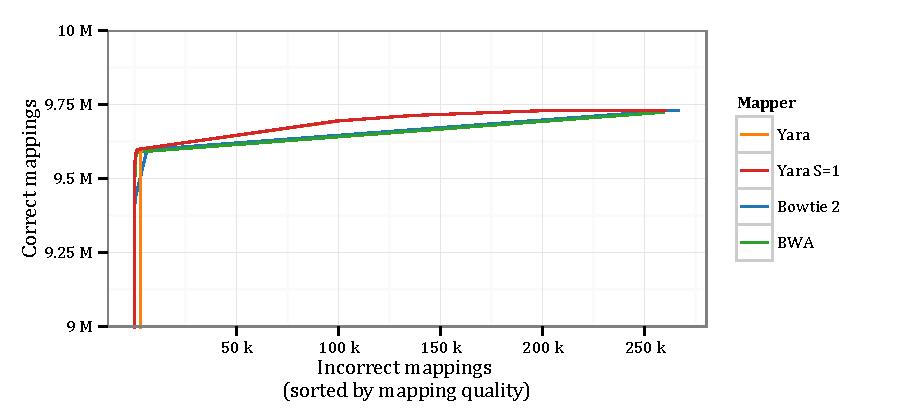
\includegraphics{hiseq_hg19_like_se.accuracy.pdf}
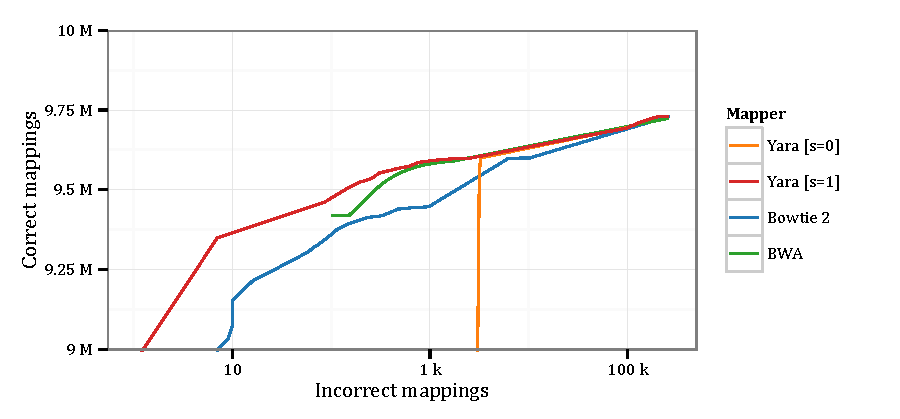
\includegraphics{hiseq_hg19_like_se.accuracy.log.pdf}
\end{center}
\end{figure}

%\begin{figure}[t]
%\begin{center}
%\caption[Yara throughput results on simulated single-end data]{Yara throughput results simulated single-end data.}
%\label{fig:yara:throughput-se}
%\end{center}
%\end{figure}

\begin{figure}[t]
\begin{center}
\caption[Yara accuracy results on simulated paired-end data]{Yara accuracy results on simulated paired-end data.}
\label{fig:yara:accuracy-pe}
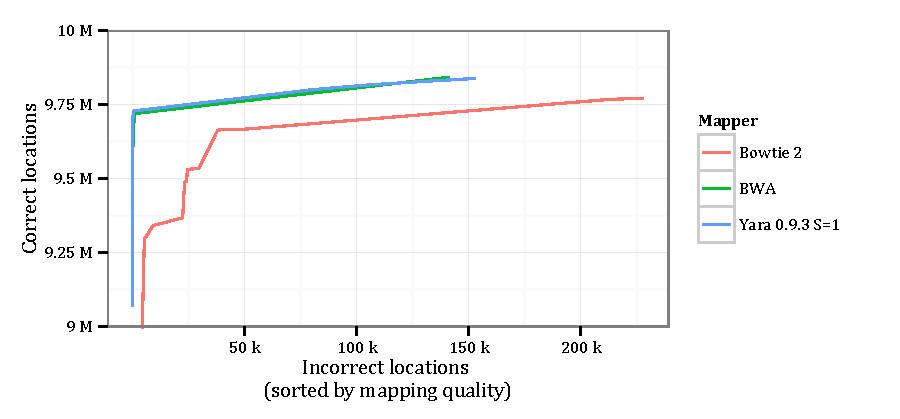
\includegraphics{hiseq_hg19_like_pe.accuracy.pdf}
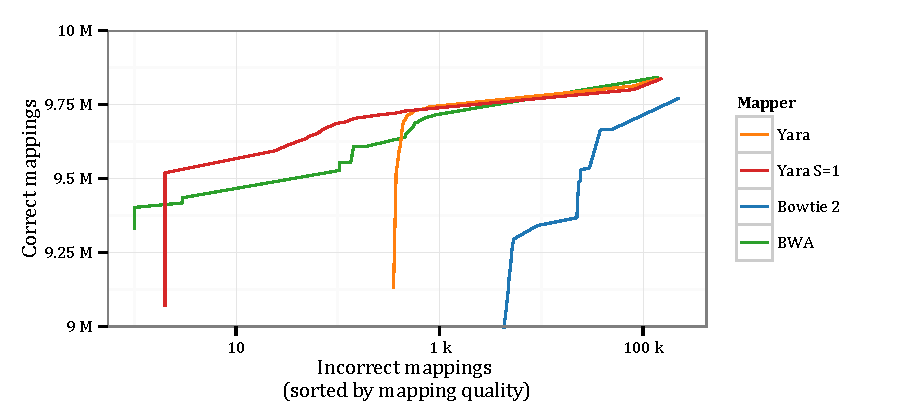
\includegraphics{hiseq_hg19_like_pe.accuracy.log.pdf}
\end{center}
\end{figure}

Comment accuracy.

Comment throughput.

\subsection{Variant calling on real data}

The last experiment assesses the performance of the same variant calling tool applied to the output of various best-mappers.
The evaluation consists of comparing the variants called by each pipeline to a set of high-confidence, single-nucleotide polymorphism (SNP) and INDEL calls provided by the \emph{Genome in a Bottle} (GIAB) consortium \cite{Zook2014}.
Thus, this experiment uses well-characterized datasets to estimate both true-positive and false-negative rates of each best-mapper within variant calling pipelines.

The GIAB consortium provides a set of calls (NIST v2.18) for the pilot genome NA12878.
Thus, this experiment applies all variant calling pipelines on an exome re-sequencing (SRA/ENA id: SRR1611178) of the same NA12878 individual.
Such sequencing run, produced by the XXX Institute, consists of $2 \times 100\,\text{bp}$ Illumina HiSeq 2000 reads and has a mean coverage of $150$~x.

As variant caller, this experiment adopts the widely used \emph{GATK Unified Genotyper} (UG), which calls both SNVs and INDELs.
According to the GIAB guidelines, the evaluation first decomposes complex variants using the tool \emph{vcfallelicprimitives} and subsequently compare called variants to the set of trusted variants using the tool \emph{UGene XXX}.
This last tool counts the number of correct and incorrect variants, stratifies them by variant quality, and reports their cumulated counts.
The output of the evaluation is plotted as ROC curves in figure~\ref{fig:yara:calling-snps}.

\begin{figure}[t]
\begin{center}
\caption[SNPs calling accuracy results]{SNPs calling accuracy results.}
\label{fig:yara:calling-snps}
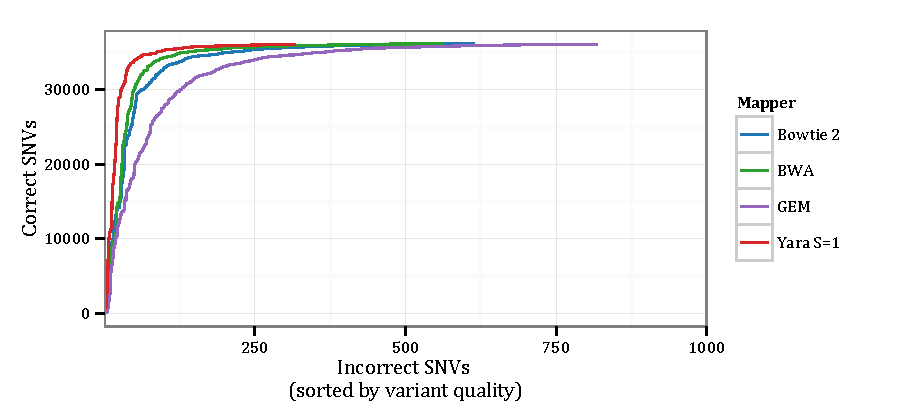
\includegraphics{SRR1611178.snp.pdf}
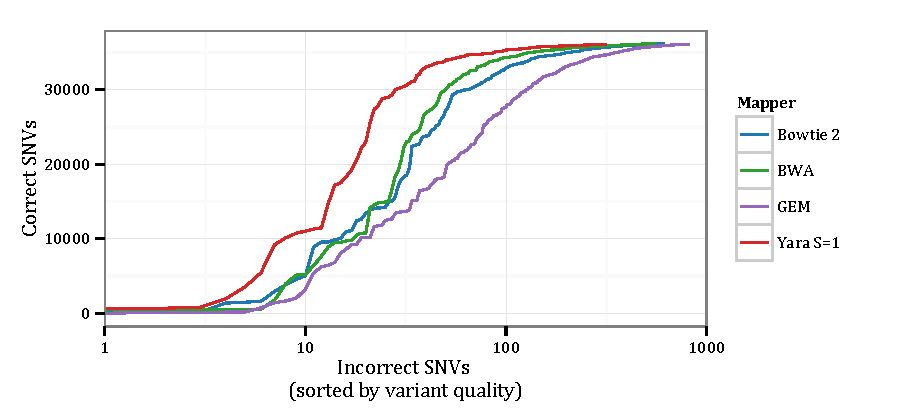
\includegraphics{SRR1611178.snp.log.pdf}
\end{center}
\end{figure}

\begin{figure}[t]
\begin{center}
\caption[INDELs calling accuracy results]{INDELs calling accuracy results.}
\label{fig:yara:calling-indels}
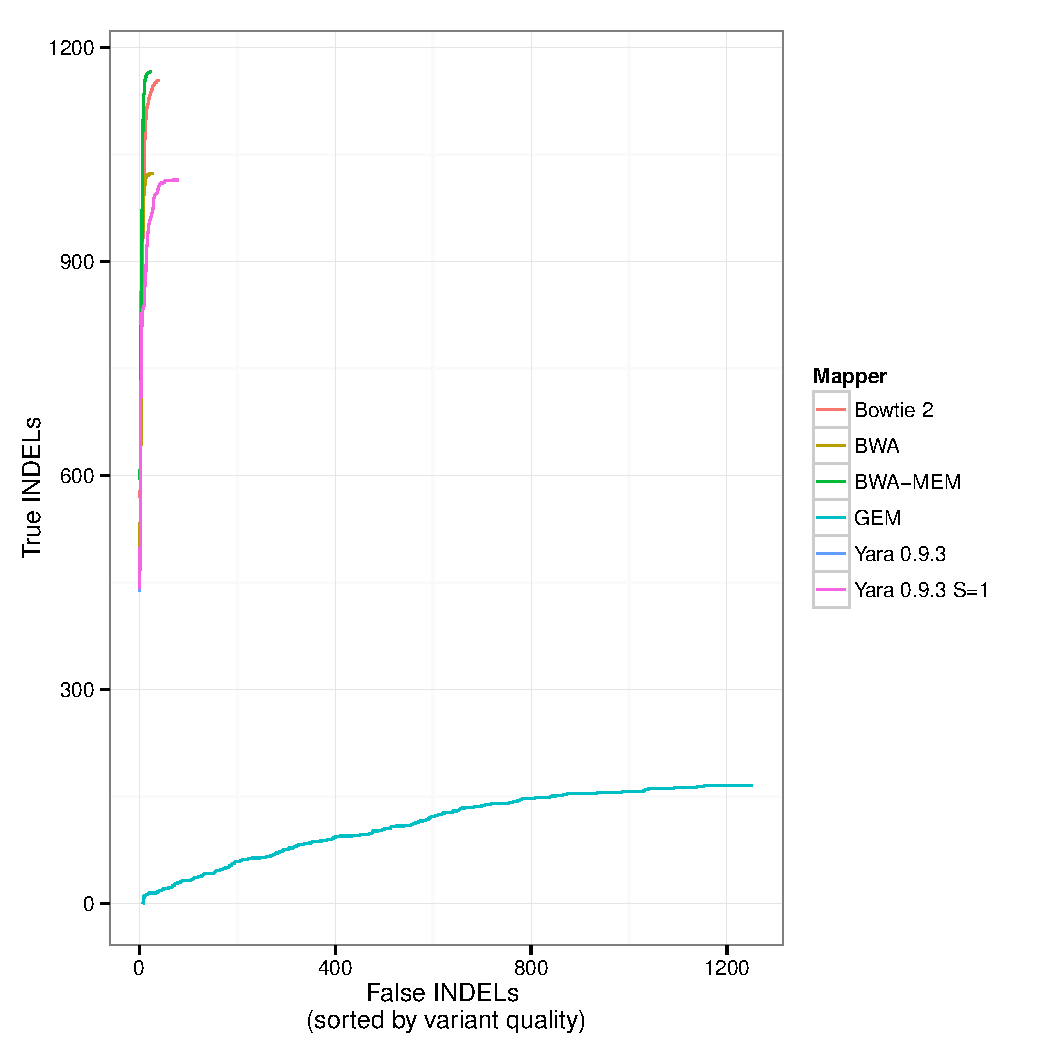
\includegraphics{SRR1611178.indel.pdf}
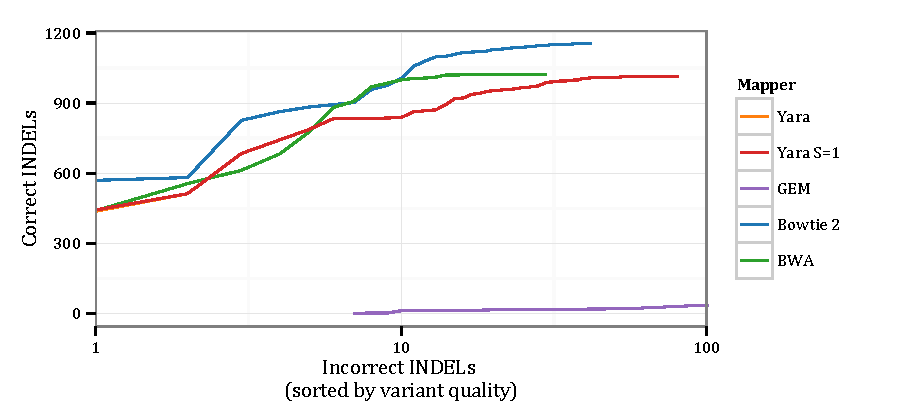
\includegraphics{SRR1611178.indel.log.pdf}
\end{center}
\end{figure}

Comment accuracy.

Comment throughput.


% -----------------------------------------------------------------------------

%\section{Discussion}

%Yara does not consider local alignments and chimeric reads.
